\subsection{会員機能}
会員機能は，以下のような機能から構成されている．

\begin{itemize}
    \item 新規会員登録
    \item ログイン・ログアウト
    \item 退会
    \item 問い合わせ
    \item 事業者申請機能
\end{itemize}


\subsubsection{新規会員登録}

一般会員が新規会員登録として，Googleアカウントを用いて会員になる機能．

利用規約に同意し，「Googleでログイン」を選択すると，Google認証に移る．
次に，登録するアカウントを選択，そのアカウント情報をDBに格納する．
これでログインが完了し，ホーム画面に遷移する．

\begin{figure}[H]
        \centering
        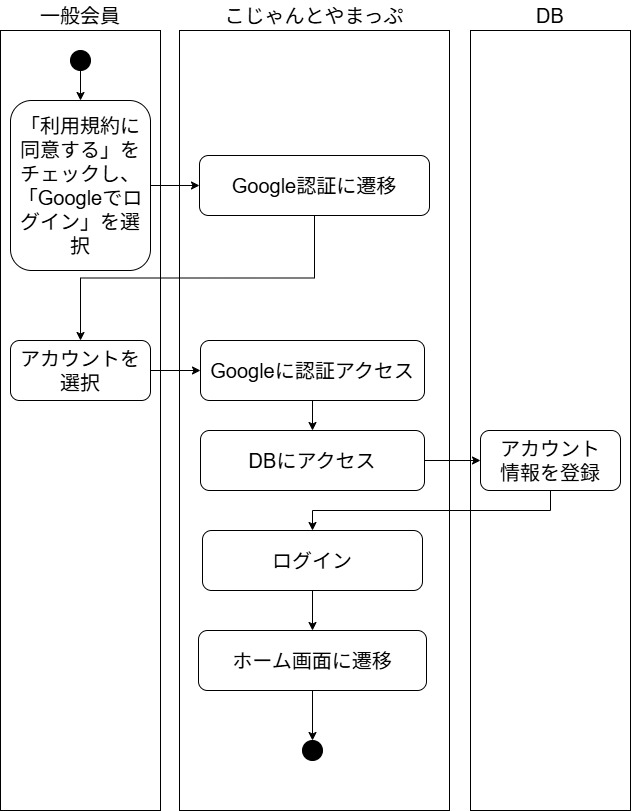
\includegraphics[scale=0.5]{sections/fig_account_general/account_gen1.jpg}
        \caption{新規会員機能}

        %\label{}

\end{figure}

\subsubsection{ログイン・ログアウト}
一般会員がGoogle認証を用いて、任意にログイン・ログアウトを行う機能．

ログイン機能では，一般会員が Google アカウントを用いた認証によってシステムにログインする．
ログインの処理は新規会員登録時の認証手順とほぼ同様であり，ログイン認証画面で取得したアカウント情報が
データベースに登録済みである場合にログインを許可する．

\begin{figure}[H]
    \centering
    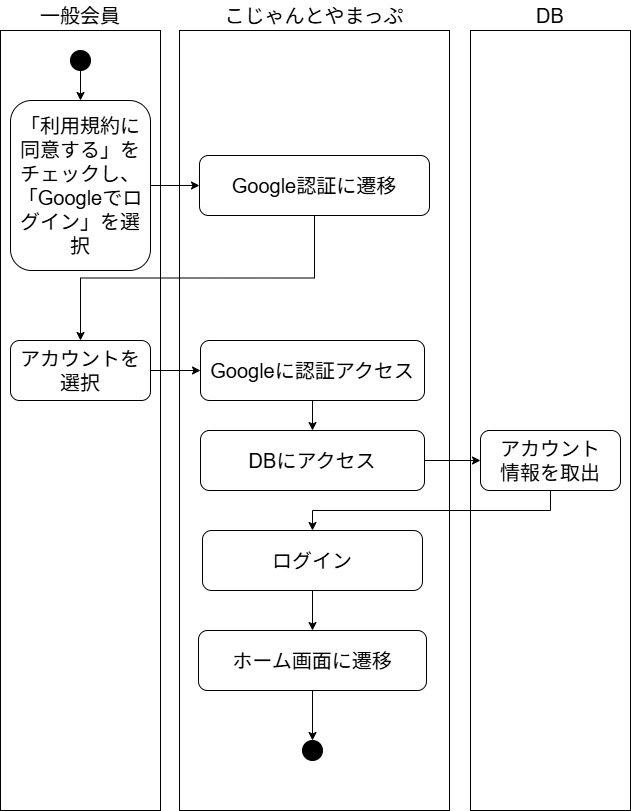
\includegraphics[scale=0.5]{sections/fig_account_general/account_gen2_1.jpg}
    \caption{ログイン}
    %\label{fig:pinpost_bus1_1}
\end{figure}

ログアウト機能では，すでにログインしている会員が任意のタイミングでログアウト操作を行うことができる．
ログアウト操作時にはまずログアウト画面を表示し，ユーザがキャンセルを選択した場合はホーム画面へ戻る．
ログアウトを確定した場合はセッション情報を無効化し，ログイン画面へ遷移する．


\begin{figure}[H]
    \centering
    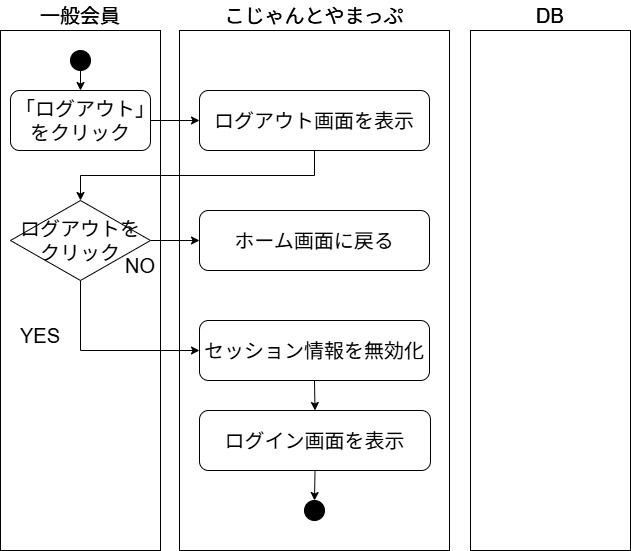
\includegraphics[scale=0.5]{sections/fig_account_general/account_gen2_2.jpg}
    \caption{ログアウト}
    %\label{fig:pinpost_bus1_1}
\end{figure}

\subsubsection{退会}

\subsubsection{問い合わせ}

\subsubsection{事業者申請機能}



